\section{Component view}
\label{sec:component_view}
\begin{figure}[ht]
    \centering
    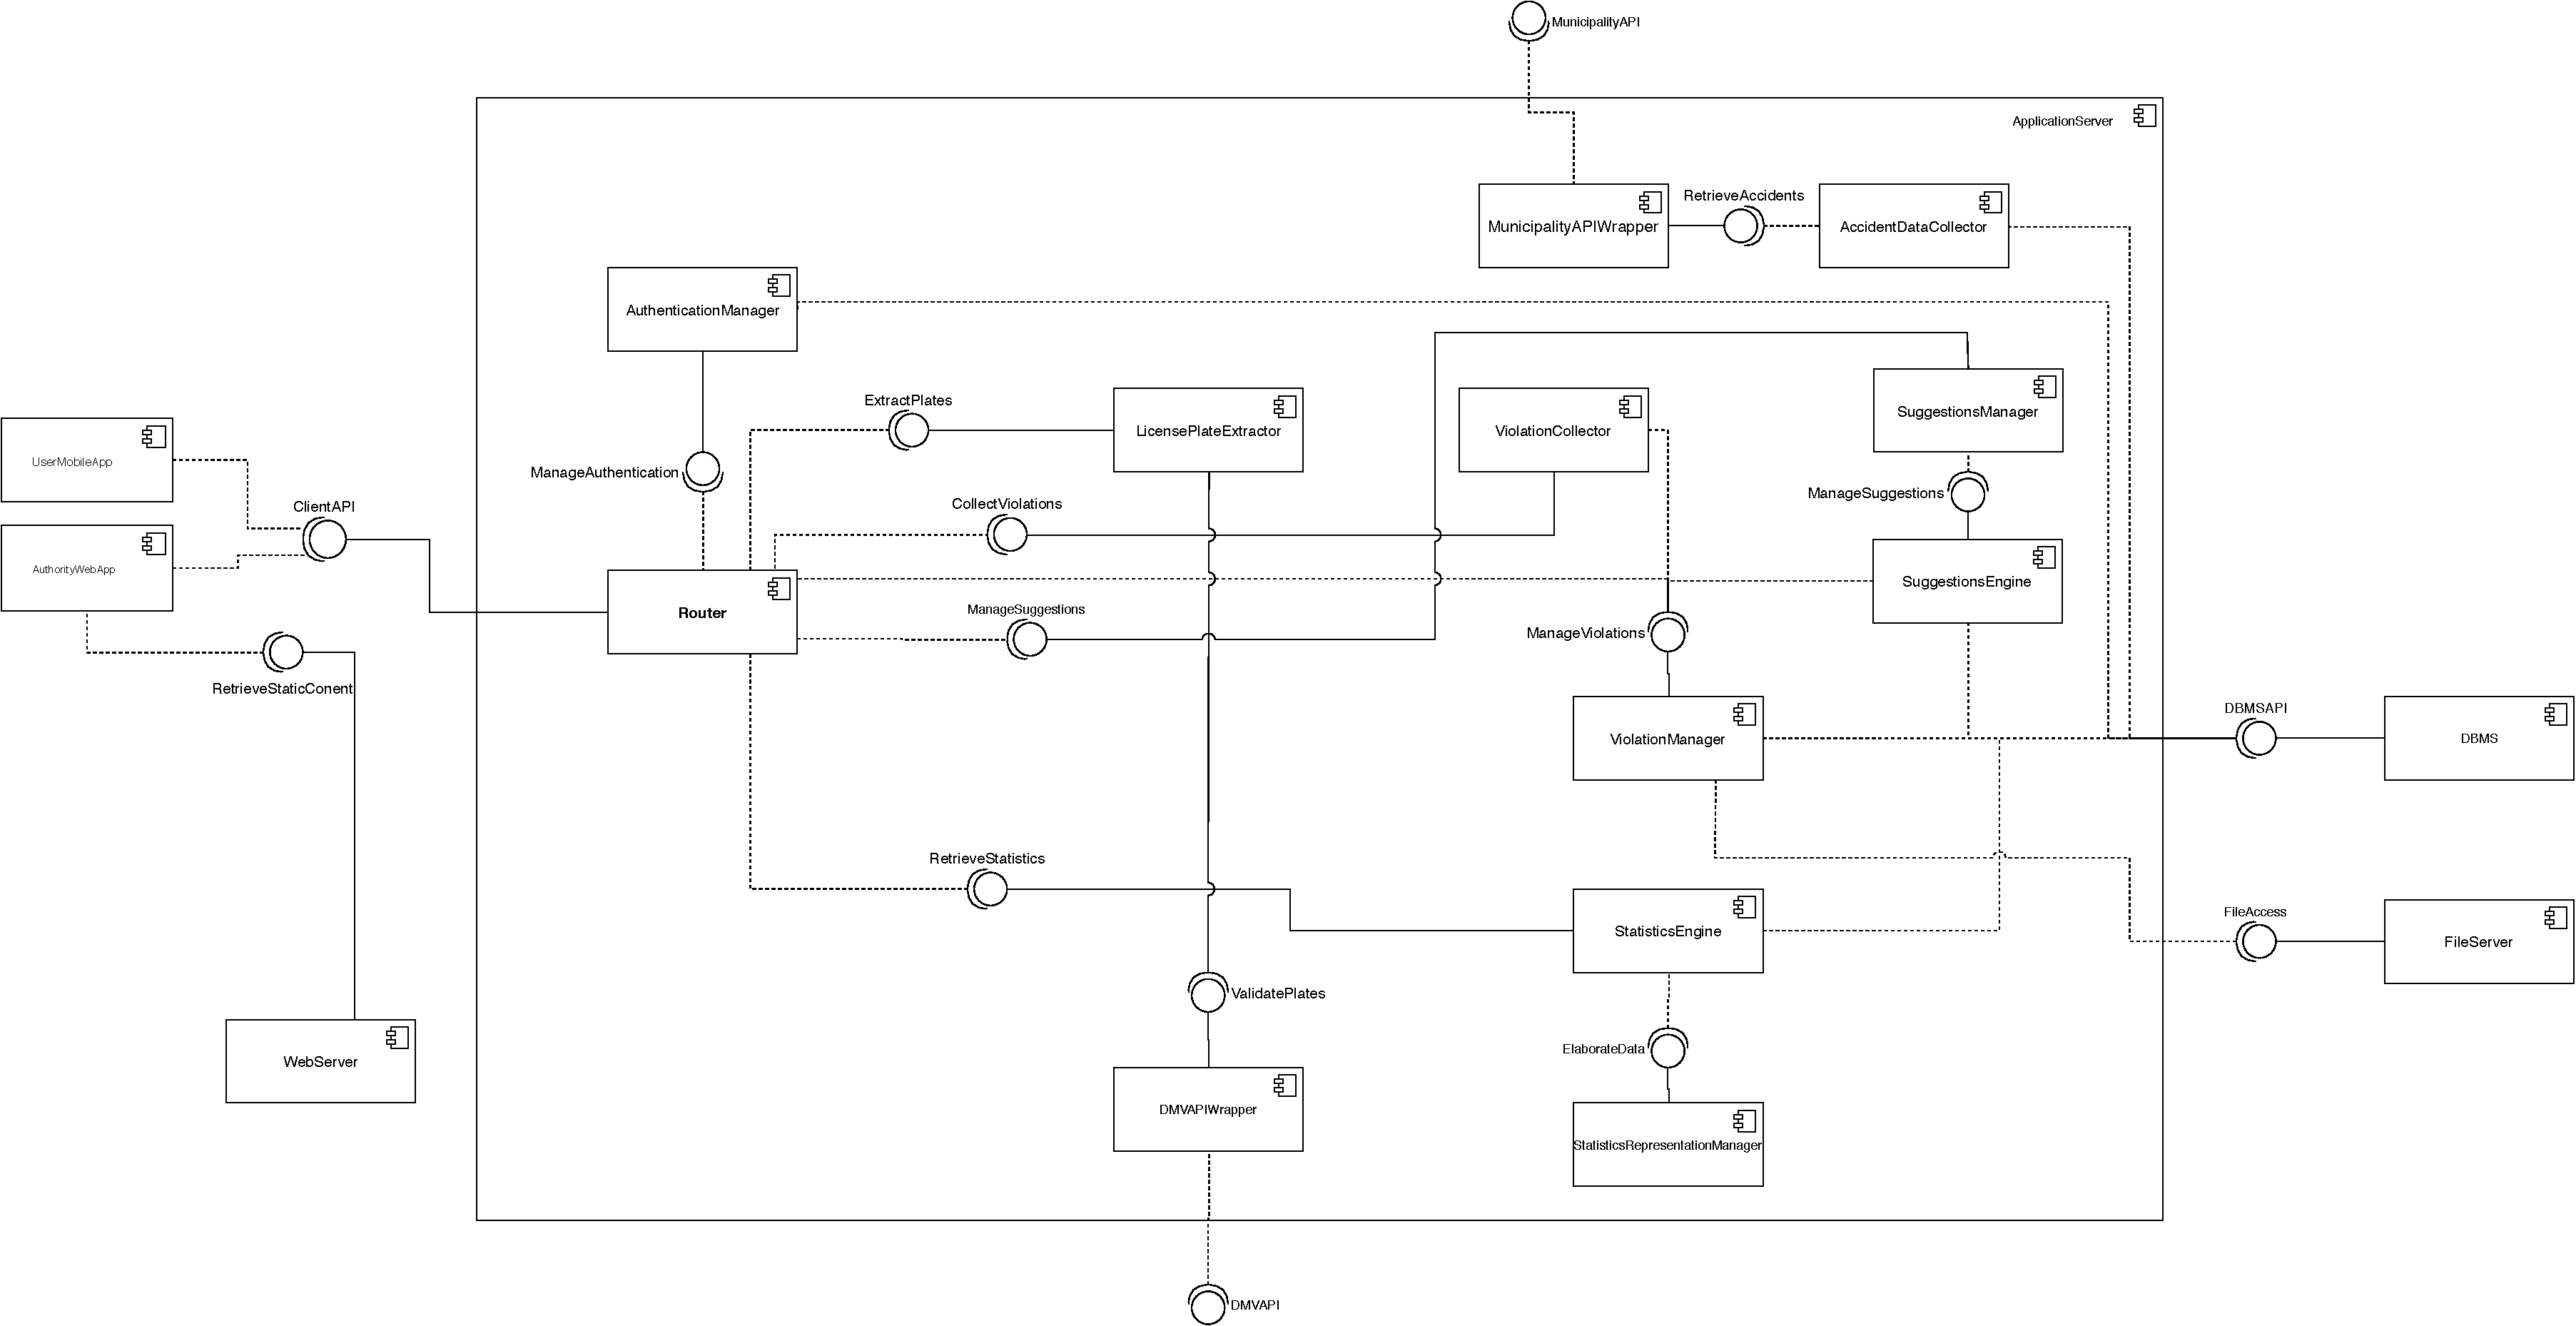
\includegraphics[width=\textwidth]{dd_component.pdf}
    \caption{Component Diagram, with an exploded view of the ApplicationServer
    subsystem.}
    \label{fig:component_diagram}
\end{figure}
\noindent
The system is composed of four subsystems:
\begin{description}
    \item[UserMobileApp] This is the smartphone app that provides all the
    functionalities to the citizens. It handles the presentation and the user
    interaction locally, while it interacts with the application server
    by using the \emph{ClientAPI} (RESTful).
    \item[AuthorityWebApp] This is the web application used by authorities.
    It handles the presentation and user interaction. The data to be displayed
    is retrieved using the REST API provided by the application server
    (\emph{ClientAPI}).
    \item[WebServer] This is a web server that provides static assets for the
    \emph{AuthorityWebApp}, such as HTML documents, the JavaScript code that
    runs the web app, CSS stylesheets and static images such as icons, etc.
    In this way web server replicas can be brought up or down depending on the
    current load. Since the replicas are all equal and completely stateless,
    each request can be equivalently routed to any of them.
    The only occasion in which the replicas must be synced is when a part of
    the web app code (or other asset) is changed, which can be considered a
    maintenance operation.
    \item[ApplicationServer] This is the component responsible for carrying
    out the business logic of the system. The application data related to
    SafeStreets is stored and retrieved from a relational DBMS.
    The component also accesses a file server to store and retrieve the images
    of the reported violations.
    Finally, it uses the interfaces offered by the Department of Motor Vehicles
    (\emph{DMVAPI}) and the various municipalities (\emph{MunicipalityAPI}).
    \item[DBMS] This component is the central relational database, used by the
    ApplicationServer. It stores all the application data that needs to be
    persisted (users, violations, retrieved accidents, municipality and
    authority info, access tokens), except the actual pictures of the
    violations. Of course, this component must not be implemented from scratch,
    but we just need to choose a commercially available solution that meets the
    requirements and configure it. It is required for the DBMS to support
    \emph{distribution} with a single transaction manager and also working with
    \emph{geographical data types}, to speed up queries based on locations.
    \item[FileServer] It is only responsible to store the images attached to
    the violation reports and making them available to be retrieved by the
    clients via the REST API.
\end{description}

\noindent
In figure \vref{fig:component_diagram} we further detail the internal components
of the \emph{ApplicationServer} subsystem, which is the core of the system.
Here we also provide a description of the various components and their
interactions:
\begin{description}
    \item[Router] This component exposes a public REST API, named
    \emph{ClientAPI} shared between the mobile and the web clients, which they
    use to perform all requests to the server (authentication and dynamic data
    in general). Each request type is assigned to a different REST endpoint
    (identified by an URL) and is then routed to the appropriate component,
    which will then carry it out autonomously and respond to the client
    (if required).
    \item[AuthenticationManager] It is responsible for the registration and
    login of both citizens and authority operators. Since it has to read and
    write user data, it needs to interact wit the \emph{DBMS}.
    This component is also responsible for handling sessions: after a successful
    login the component generates an \emph{access token} for the specific user,
    which is valid for a limited time. The token is then stored in the DB
    and can be accessed by the other components and finally it gets sent to the
    client that sent the login request.
    Now, when the client makes a request, it also provides the token which will
    be checked against the DB by the component that will handle the request.
    \item[LicencePlateExtractor] This component receives violation photos
    uploaded by the users and tries to extract the biggest licence plate
    number it an find in the photo. Then it checks if the detected plate exists
    by using the DMV API. If a valid licence plate number has been extracted,
    the component sends it to the client as a response, so it can autocomplete
    the licence plate field in the request report.
    This task has been separated from the violation reporting to take load
    off from the \emph{ViolationCollector} and also to give users the ability
    to manually insert the licence plate number if it couldn't be detected or
    to correct it.
    \item[ViolationManager] This component provides primitives to store,
    retrieve and review violations (i.e. mark them as accepted or discard them).
    It is used by the ViolationCollector to store an incoming violation and in
    this regard it is responsible to check and assign it to a responsible
    authority, based on the municipality in which the violation occurred. If
    this fails, the violation cannot be stored. Storing the violation also
    includes saving its attached photo to the \emph{FileServer}.
    In turn, when an operator requests to review violations, this components is
    activated and it is responsible to only retrieve the violations assigned to
    the requesting authority and sending them as a response.
    When the operator decides to mark a violation as accepted or discarded, this
    component is responsible for applying the change in the DB; note that it is
    necessary to check that the violation was assigned to the requesting
    authority by using the access token provided with the request.
    \item[ViolationCollector] This component is responsible to handle incoming
    violation reports from the users, in particular to check their validity and
    then use the \emph{ViolationManager} to store them in the DB.
    In particular, it checks that the report contains all the required fields
    and that the licence plate number is valid (by using the DMV API).
    \item[StatisticsEngine] This component is responsible for computing
    statistics for both users and authorities. A statistics request will come
    in, indicating the type of statistics (e.g.\ violations per month) and
    possibly various filters (e.g.\ municipality, year, \dots); the component
    will perform a query to the DB and compute the required statistics.
    These are then passed on to the \emph{StatisticsRepresentationManager}
    and the result is sent as a response to the client.
    \item[StatisticsRepresentationManager] Given some \emph{raw} statistics,
    this component is responsible to generate their appropriate representation
    to be fed to the client libraries used to show statistics.
    This takes into account the diagram colors, text labels, measurement units
    and all the parameters needed by the client libraries to visualize the
    appropriate diagram.
    The reason for this to be done server-side is that we don't have to send
    raw data over the network and we can provide a consistent representation
    between the mobile app and the website (in terms of colors, labels, etc.).
    \item[AccidentDataCollector] This component is responsible for periodically
    collecting data about accidents from the municipalities that provide it
    and store it to the database. As we stated in the RASD, we assume that the
    municipalities provide an API to retrieve all accidents that have been
    registered after a certain date; the component can rely on this to perform
    incremental updates, rather than retrieving all the data each time.
    Since the accident data will be used to compute suggestions, a task that
    requires a lot of accesses, we chose to store it locally rather than
    continuously contacting the municipality API. This is also dictated by
    the fact that we have no control over the availability of the external
    data sources.
    \item[SuggestionsEngine] This component is responsible to periodically
    compute new suggestions for the authorities that have activated the
    \emph{SmartSuggestions} functionality.
    It reads data about violations and accidents directly from the DB and
    then computes the suggestions by using Machine Learning algorithms.
    These suggestions are then stored into the DB, so they can be retrieved
    by the authority. Note, however, that no notification is actively sent to
    the authority.
    Furthermore, since there can be a lot of municipalities involved, the
    component should also be able to schedule its jobs over time, in order to
    keep up to date with new violations and accidents data.
    \item[SuggestionsManager] Provides methods to retrieve suggestions and
    mark them as carried out. Analogously to \emph{ViolationManager} it receives
    requests by authority web apps containing an access token, and it has to
    allow access only to the suggestions for the authority that owns the token.
    \item[DMVAPIWrapper] The components that need to check the validity of
    a licence plate number don't directly interact with the external API, but
    with this internal component that wraps around the API.
    For details on the advantages of this approach
    see~\ref{subsec:adapter_pattern}
    \item[MunicipalityAPIWrapper] Similarly to the previous one, we provide a
    wrapper also for the APIs offered by municipalities to retrieve data about
    accidents. Here the need for a component that converts the various data
    formats provided by the external APIs to an internal, shared format is
    even more evident, since it is quite unlikely that all the municipalities
    provide such data in the same format.
\end{description}